\documentclass[../main.tex]{subfiles}

\begin{document}

    Over the last decades, information technology has been constantly evolving.
    With the concept of virtualization and the increased accessibility of computing resources through \gls{cloud} platforms, \gls{cloud_computing} has become a topic of interest.
    However, as with everything in \acrfull{it}, it takes a long time to go from inception to wide adoption.
    Today, the whole industry is adopting \gls{cloud_computing} as part of the digital transformation.

    \subsection{Current trend}
    \label{subsec:intro-trend}

    The current trend in the market is strongly geared towards \acrfull{ai}, \gls{cloud} and \gls{devops}.
    This thesis focuses on concepts around \gls{cloud} and \gls{devops}.

    Comparing the \gls{google_trends} of the major \gls{public_cloud} providers worldwide, namely \gls{microsoft_cloud}, \acrfull{gcp}, \acrfull{aws}, Alibaba Cloud, IBM Cloud and Oracle Cloud, clearly shows strong development in interest over the past ten years (Fig.~\ref{fig:cloud_trend_world}).
    \gls{google_trends} show the relative demand of a given topic based on Google search results.
    Although not every provider is recording the same prosperity, there is certainly big demand and even bigger competition.

    \begin{figure}[h]
        \centering
        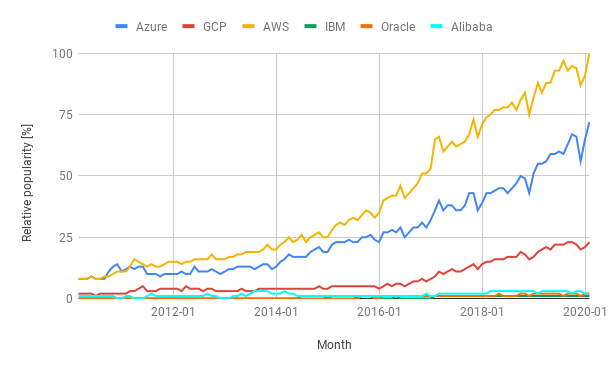
\includegraphics[width=.8\linewidth]{img/intro_cloud_trend_world.png}
        \captionsetup{justification=centering}
        \caption{
        Comparison of \gls{google_trends} on \acrshort{aws} (yellow), \glsdisp{microsoft_cloud}{Azure} (blue), \acrshort{gcp} (red), Alibaba Cloud (cyan), Oracle Cloud (orange), and IBM Cloud (green).\cite{cloudtrend_world, cloudtrend_world_2}
        }
        \label{fig:cloud_trend_world}
    \end{figure}

    When limiting the statistics to Switzerland, \gls{microsoft_cloud} takes the lead.
    The \gls{google_trends} comparison shows the three major \gls{public_cloud} providers, \glsdisp{microsoft_cloud}{Azure}, \acrshort{gcp} and \acrshort{aws}, and the major Swiss-native \gls{cloud} provider Swisscom (Fig.~\ref{fig:cloudtrend_swiss}).
    \glsdisp{microsoft_cloud}{Azure}'s lead in Switzerland could be related to Microsoft's strong presence in Switzerland for over 30 years and collaboration with many companies including Swisscom.\cite{microsoft_exand_swiss}

    \begin{figure}[h]
        \centering
        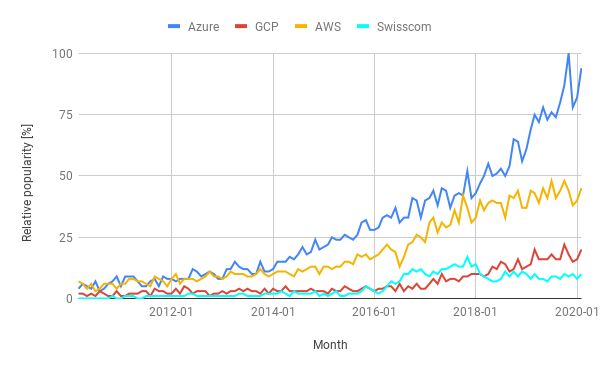
\includegraphics[width=.8\linewidth]{img/intro_cloud_trend_swiss.png}
        \captionsetup{justification=centering}
        \caption{
        Comparison of \gls{google_trends} on \glsdisp{microsoft_cloud}{Azure} (blue), \acrshort{aws} (yellow), \acrshort{gcp} (red) and their Swiss competitor Swisscom (cyan).\cite{cloudtrend_swiss}
        }
        \label{fig:cloudtrend_swiss}
    \end{figure}

    \begin{figure}[h]
        \centering
        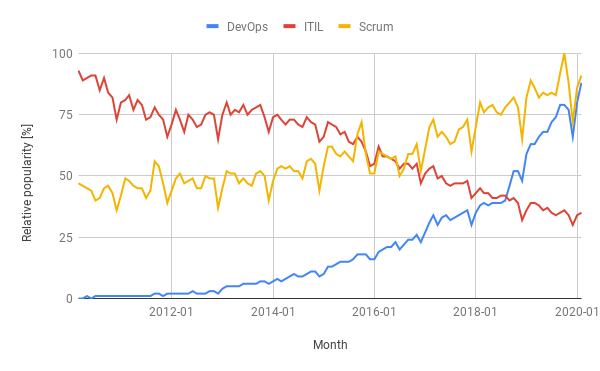
\includegraphics[width=.8\linewidth]{img/intro_devops_trend.png}
        \captionsetup{justification=centering}
        \caption{
        \gls{itil} (red) in contrast to \gls{devops} (blue) and \Gls{scrum} (yellow) on \gls{google_trends}.\cite{devopstrend}
        }
        \label{fig:devops_trend}
    \end{figure}

    \Gls{cloud} platforms are an enabler for \gls{devops} as they offer an abstraction over common \acrshort{it} infrastructure and as a result reduce operational workloads for the user.
    Therefore, it is no surprise that the \gls{devops} trend has evolved very similarly to the \gls{cloud} trend.
    Contrasting \gls{devops} with \gls{itil} on \gls{google_trends} illustrates how the paradigm shifts.
    \gls{itil} is a common framework for software delivery and change management.
    While \gls{itil} was rather management driven, \gls{devops} together with \Gls{scrum} now takes precedence as the industry is adopting more agile, development-centric methodologies (Fig.~\ref{fig:devops_trend}).

    All of the above comparisons are based on \gls{google_trends} statistics, which limits the scope of data to a single search engine.
    While the Google search engine is widely used, this limitation has to be considered when drawing any conclusions on the data presented.

    \subsection{How the industry adapts}
    \label{subsec:intro-industry}

    Netflix is one of the pioneers in successfully applying \gls{devops} with what they called full cycle developers.
    Today, they are not only famous for their seamless streaming experience, but also for world class engineering.\cite{netflix_blog_fcdev}

    Walmart, mostly known for their grocery stores, acquired and open-sourced their own \gls{devops} platform which they use to run their e-commerce presence.\cite{walmart_blog_oneops}

    However, not all Fortune 500 companies have been keeping up with the same pace as Walmart and Netflix.
    Taking a glance at the financial sector, banking corporations hold a vast technology legacy that not only manages the majority of all wealth, but also handles millions of transactions every day which are crucial to the economy.
    The imposition of restrictions and regulations on financial institutions due to their significance for the economy makes it especially challenging to be efficient and therefore requires a mature operation model to remain competitive.
    Fortunately, this has been acknowledged by the industry and corporations such as UBS Group and ING Group are starting to invest more into digital transformation.
    This includes adoption of agile methodologies but also \gls{devops} practices.
    After all, they are becoming technology companies that offer financial services.\cite{ing_blog_agile,infoq_ubs_agile}

    Looking at the country with the biggest relative population in the world, China, the majority of citizens use Wechat Pay or Alipay for payments.
    Both services are owned by technology companies that do not originate in the financial sector.\cite{payment_china}

    Fintech company and neo-bank Revolut has acknowledged the need for a mobile-first banking experience and managed to gain 12 million customers in only a few years.
    The fintech market is growing and Revolut is only one of many players offering attractive services to their clients.
    But it is not only the modern, technology-driven appearance that makes the difference.
    Fintech start-ups are much more efficient in developing new products as they do not have to deal with legacy technology and heavy bureaucracy.
    With big tech giants starting to expand into the financial sector, the competition gets even bigger, leaving traditional financial institutions with no other option but to catch up on technology and innovation.\cite{revolut,fintech_pressure,bigtech_fin_pressure}

    For cultural and historical reasons, using and contributing to open-source software has not been promoted in the area of financial business.
    The use of closed-source and proprietary software has been deemed advantageous for legal, compliance and competitive reasons.
    As more fintech and technology-driven companies are entering the market, a more collaborative culture manifests, trying to provide standard and open-source platforms through foundations and initiatives, such as FINOS and the open banking project.\cite{fin_oss_myths,openbanking}

    \subsection{Problem statement}
    \label{subsec:intro-statement}

    Nowadays, every company is faced with digital transformation.
    Moving software estate to the \gls{cloud} is inevitably part of it.
    In that process, companies will probably start off with a \gls{hybrid_cloud} model, even if the goal is to move completely to the \gls{public_cloud}.

    This thesis aims to highlight challenges for companies deploying their applications to the \gls{cloud} and develop a \gls{hybrid_cloud_ops} solution that enables the adoption of a \gls{hybrid_cloud} model following a \gls{devops} approach.
    As maintenance of existing non-\gls{cloud_native}, legacy applications is deemed pertinent to large enterprises, the thesis slightly deviates from the initial assignment and includes concepts of how to integrate an existing legacy stack with a modern \gls{hybrid_cloud_ops} model.

    \subsection{Thesis contributions}
    \label{subsec:contributions}

    The main contribution of this thesis is a novel and simple way of \gls{hybrid_cloud} management based on the container orchestration system \gls{kubernetes} that provides a tag-based support model and a policy-driven continuous deployment workflow which can be integrated with an existing legacy \acrshort{it} stack consisting of non-\gls{cloud_native} applications.
    It reuses existing \acrshort{api} definitions with standard protocols to enable declarative management of resources with minimal overhead and is not bound to any \gls{kubernetes} distribution or hosting.
    It can therefore be applied to any \gls{cross_cloud} deployment model that is based on \gls{kubernetes}, including \gls{multi_cloud}.

    In addition, a high-level plan is provided for a comprehensive \gls{hybrid_cloud_ops} model for future work as extension of the elaborated concepts.

    As further contributions, a collection of books and papers related to the discussed topics and a visual overview of the current state of \gls{devops} interpretations is provided.

    \subsection{Thesis overview}
    \label{subsec:thesis-overview}

    This section provides a brief overview of this thesis and its sections as outlined in the table of contents.

    \textbf{Definitions}
    sets the theoretical basis and expands on the terms \gls{cloud} and \gls{devops}.

    \textbf{Concepts}
    delineates the work, refines the problem statement and introduces the concepts which are implemented and evaluated as part of this thesis.

    \textbf{Methodology}
    describes the scientific methods used to evaluate the concepts, which is an assessment by an expert group and experimentation based on the conceptual work.

    \textbf{Instrumentation}
    describes the instruments used and developed to compute the results.
    It describes the concrete implementations on a technical level.

    \textbf{Results}
    presents the results that have been produced using the methodology and instrumentation.

    \textbf{Discussion and Outlook}
    reflects on the problem statement and concepts based on the results and discusses the impact and relevance of the work.
    Furthermore, it expands on the idea of a comprehensive \gls{hybrid_cloud_ops} model as part of future work and comes up with recommendations for enterprises.

\end{document}

